\cleardoublepage

\section{实验}
\subsection{实验环境}
本次实验研究的是在Linux+Anaconda+Pytorch的环境下进行的。

Linux是一种自由和开放源码的类Unix操作系统,相较于另一个操作系统window,在Linux系统上运行神经网络有诸多优势。
首先是易用性强,window系统很多时候对硬件有较高要求,而Linux系统即使在低成本设备上也高度稳定,此外丰富且强大的
终端工具,使得执行效率大幅提升。其次是较快的配置速度,现阶段的深度学习个人开发环境依赖GPU,在Linux系统
上配置底层硬件,比window要容易快速得多。再者,是更好的生态,得益于Linux是一个开源的系统,它有更多深度学习框架
的官方支持,tensorflow,torch,docker等社区都是优先支持Linux。

Anaconda是一个免费开源的Python的发行版本,可以完成计算科学的各种任务。Anaconda主要解决了官方Python的两个问题。
其一,提供了强大的包管理功能,在数据分析中会使用很多第三方的包,conda(anaconda中的一个包管理器)可以为安装和
管理这些包提供帮助,包括安装、卸载和更新包。其二,提供了有效的环境管理功能,由于python版本的兼容
性问题,同时使用Python2和Python3容易造成许多混乱和错误,anaconda能够解决多版本Python并存、切换的问题。

Pytorch是一个GPU加速和自动求导的深度学习框架,可完成一些深度学习的任务。使用Pytorch主要出于两点考虑。一个方面是,
Pytorch使用动态图进行运算,和使用静态图计算的TensorFlow相比,动态图的运行机制更适合研究者调试。另一个方面是,Pytorch
的代码相对易写,pytorch的编码要求和python一致,可以像写python代码一样设计深度学习模型,而使用TensorFlow则要求使用
契合它的API,这相对来说比较复杂。

\subsection{数据集}
本次实验,我们的主要任务是节点级别的分类任务。对于一个给定的网络,我们已知它的图结构,它的部分节点已经被标记,部分节点未
被标记。图卷积神经网络可以通过学习出一个鲁棒模型,来有效地识别未标记节点的类标记。为此,可以通过叠加图卷积层,然后再叠
加一个用于多分类的softmax层,来构建一个端到端的网络。图\ref{1-2}就展示了这样的例子。

本次研究使用当前比较流行的Cora、Citeseer、Pubmed数据集来进行实验,见表\ref{tabel4-1}。这三个数据集都是来自引文网络,主要任务是论文的分类(即
节点级分类的半监督学习),标签率是实验中有标签的节点和总节点数量的比值。引文网络就是由论文和他们的关系构成的网络,这些关系包括例如
引用关系、共同的作者等,具有天然的图结构。

\begin{table}[]
    \centering
    \caption{数据集统计表}
    \label{tabel4-1}
    \begin{tabular}{lllllll}
    数据集      & 类别   & 节点的数量 & 边的数量  & 标签的种类 & 特征维度 & 标签率   \\ \hline
    Citeseer & 引文网络 & 3327  & 4732  & 6     & 3703 & 0.036 \\
    Cora     & 引文网络 & 2708  & 5429  & 7     & 1433 & 0.036 \\
    Pubmed   & 引文网络 & 19717 & 44338 & 3     & 500  & 0.003
    \end{tabular}
\end{table}

以Cora数据集(图\ref{4-1})为例,Cora数据集由许多机器学习领域的论文构成,总共有2708篇论文,这些论文被分为7个类别。每一篇论文至少引用了
该数据集里面另外一篇论文或者被另外一篇论文所引用,原论文和引用的论文构成了一条天然的边,总共有5429条边。数据集中有一个包
含多个单词的词汇表,它去除了出现频率较小的词,最终词汇表中有1433个词汇,即每篇论文的特征维度是1433,然后、、论文中是否出现了
某个词用0或1进行表示。我们实验默认已知5429条边(即已知图结构),且已知每篇论文的特征向量,知道部分论文的类别,
任务是对其他不知道类别的论文进行分类。

\begin{figure}[ht]
    \centering
    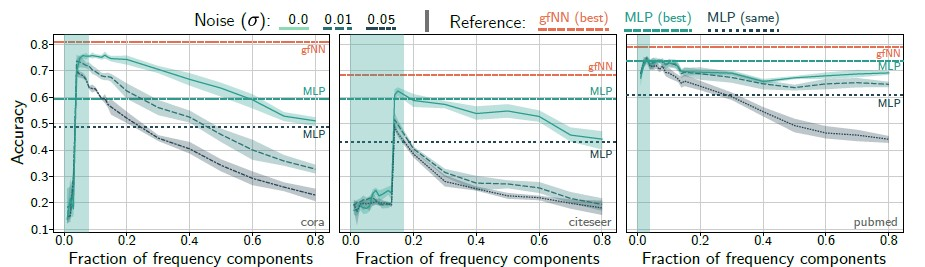
\includegraphics[width=8cm]{experiment/1.jpg}
    \caption{\label{4-1}Cora数据集可视化}
\end{figure}

\subsection{实验结果}
实验中对比的三个神经网络分别是,GAT、simple GAT、our GAT,如图\ref{4-2}所示。本部分将展示在Cora数据集上训练的实验结果,Citeseer和Pubmed
数据集的训练结果在附录1中,实验结果与Cora上类似。实验代码见附录2。
\begin{figure}[ht]
    \centering
    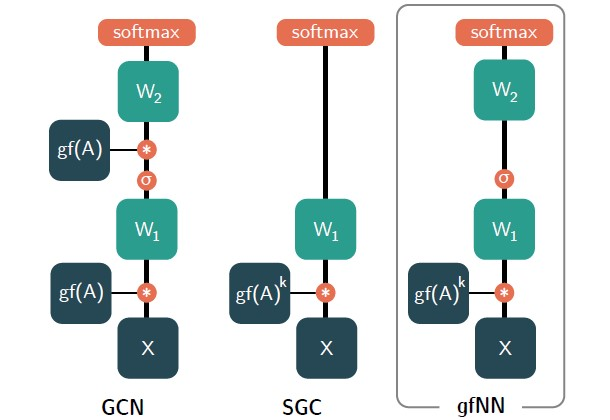
\includegraphics[width=16cm]{experiment/2.jpg}
    \caption{\label{4-2}三种图卷积神经网络结构图}
\end{figure}

\subsubsection{hop值对神经网络的影响}
第一组实验,我们对比不同hop值的图结构对GAT、simple GAT神经网络的影响。考虑到不同的隐层特征维度会有不同的实现效果,
我们将隐层的特征维度选取为效果较好时的32和64。我们考察的方面为是否出现过拟合、每epoch的训练时间、分类的准确率。
结果见表\ref{tabel4-2}。

通过分析实验结果,我们可以得到结论:GAT和Simple GAT神经网络,在图结构的hop值由1变为2时,会出现严重的过拟合现象,
并且训练效率下降,准确率下降。我们的实验也再次验证了,对于传统的GAT神经网络,不能够通过直接增加hop值来提升图卷积神经网络的
表达能力。

更进一步地分析,为何hop值的增加会对实验效果产生负面的影响,原因大致分为以下两方面。一方面,是因为注意力矩阵$A$的非
零元素过多;当图结构的hop值为1时,$A$中的非零元素只包括一阶相连的边,而图结构的hop值为2时,$A$中的非零元素还包括二
阶相连的边;与hop为1时相比,过多的元素使得在训练注意力参数$ \vec{a} $的过程中,出现过拟合现象。另一个方面,节点间边
的相连表示了他们之间的联系,但可能数据集中所有二阶相连的节点之间并不一定都有明显的关系,所以注意力矩阵$A$中非零元素的冗余,
造成了过拟合。

\begin{table}[]
    \centering
    \caption{不同的hop值对神经网络的影响}
    \label{tabel4-2}
    \begin{tabular}{|l|l|l|l|l|l|}
    \hline
                         & 图结构hop的值           & 隐层输出维度 & 过拟合 & 训练时间(ms)/epoch & 准确率(\%)      \\ \hline
    \multirow{4}{*}{GAT} & \multirow{2}{*}{1} & 32     & 不明显 & 0.45            & 85.2±0.1 \\ \cline{3-6}
                         &                    & 64     & 不明显 & 0.46            & 84.3±0.2 \\ \cline{2-6}
                         & \multirow{2}{*}{2} & 32     & 明显   & 1.05            & 77.7±0.1 \\ \cline{3-6}
                         &                    & 64     & 明显   & 1.10            & 78.5±0.1 \\ \hline
    \multirow{4}{*}{Simple GAT} & \multirow{2}{*}{1} & 32     & 不明显 & 0.19     & 80.6±0.2 \\ \cline{3-6}
                         &                    & 64     & 不明显 & 0.20            & 81.1±0.2 \\ \cline{2-6}
                         & \multirow{2}{*}{2} & 32     & 明显   & 0.42            & 78.1±0.3 \\ \cline{3-6}
                         &                    & 64     & 明显   & 0.59            & 77.6±0.2 \\ \hline                    
    \end{tabular}
\end{table}

\subsubsection{性能对比}
第二组实验,我们主要对比三种神经网络GAT、simple GAT、our GAT的性能。我们依旧将隐层的特征维度选取为32和64,考察的方面为
是否出现过拟合、每epoch的训练时间、分类的准确率。由第三章的内容我们易知,当our GAT的hop值取1时,结构上等同于simple GAT网络。
所以在本组实验中,我们将GAT和Simple GAT的hop值选取为1,将Our GAT的hop值选取为5。结果见表\ref{tabel4-3}。

实验结果表明了:我们提出的图卷积神经网络our GAT,在测试数据集上的准确率大致与传统GAT网络持平,但我们的训练效率较其提升了一倍,
训练效率大致等同于simple GAT;此外,实验过程中,我们提出的our GAT的hop值设置为5,并没有出现过拟合现象,这说明其克服了传统GAT网络
hop值只能为1的缺陷。

我们的设计思路上在实验结果上得到了验证。与GAT和simple GAT直接增加注意力矩阵$A$的hop值相比,our GAT的神经网络结构里,
$A$的hop值依然为1,我们通过矩阵多项式$ F(A) $来间接地增加图结构的hop。正是这样的设计,使得我们在几乎不影响simple GAT网络训练效率
的情况下,大大增加了其表达能力,也成功避免了过拟合;也正是因为矩阵多项式带来的表达能力的提升,我们能够将传统GAT网络中使用的两个
注意力矩阵$ A_1,A_2 $减少为一个,在不影响训练效果的前提下,提高了训练效率。

\begin{table}[]
    \centering
    \caption{三种神经网络效果对比}
    \label{tabel4-3}
    \begin{tabular}{|l|l|l|l|l|l|}
    \hline
                                & 图结构hop的值           & 隐层输出维度 & 过拟合 & 训练时间(ms)/epoch & 准确率(\%)       \\ \hline
    \multirow{2}{*}{GAT}        & \multirow{2}{*}{1} & 32     & 不明显 & 0.45           & 85.2±0.1 \\ \cline{3-6} 
                                &                    & 64     & 不明显 & 0.46           & 84.3±0.2 \\ \hline
    \multirow{2}{*}{Simple GAT} & \multirow{2}{*}{1} & 32     & 不明显 & 0.19           & 80.6±0.2 \\ \cline{3-6} 
                                &                    & 64     & 不明显 & 0.20           & 81.1±0.2 \\ \hline
    \multirow{2}{*}{Our GAT}    & \multirow{2}{*}{5} & 32     & 不明显 & 0.21           & 84.8±0.2 \\ \cline{3-6} 
                                &                    & 64     & 不明显 & 0.26           & 85.0±0.1 \\ \hline
    \end{tabular}
\end{table}

\subsubsection{hop值的选取}
\begin{figure}[ht]
    \centering
    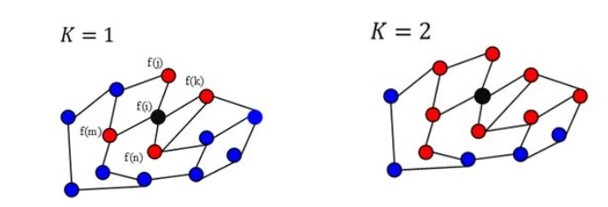
\includegraphics[width=12cm]{experiment/3.jpg}
    \caption{\label{4-3}hop值对our GAT图卷积神经网络的影响图}
\end{figure}
第三组实验,我们想要对比不同hop值,即不同的矩阵多项式的阶数K对于our GAT表达能力的影响。结果见图\ref{4-3}和表\ref{tabel4-4}。

 实验结果说明:随着K值的增加,训练时间代价略有提高,均未出现过拟合现象,测试集上的准确率先上升后不变。这是因为在K值刚开始
 增大的阶段,随着间接相连的节点关系被纳入考虑,our GAT的表达能力明显提升;而当K值较大时,K阶相连的节点数量较少,
 所以此时K值的增加对表达能力的提升不明显。K值的选取取决于数据集的特点,我们既不能选的太小,这会限制our GAT卷积神经网络的表
 达能力,也不能选的太大,这会降低训练效率。

 \begin{table}[]
    \centering
    \caption{our GAT的矩阵多项式取不同K值}
    \label{tabel4-4}
    \begin{tabular}{|l|l|l|l|l|l|}
    \hline
                             & 图结构hop的值      & 隐层输出维度 & 过拟合 & 训练时间(ms)/epoch & 准确率(\%) \\ \hline
    \multirow{12}{*}{our GAT}& \multirow{2}{*}{1} & 32     & 不明显      & 0.19           & 80.7±0.1    \\ \cline{3-6} 
                             &                    & 64     & 不明显      & 0.19           & 81.3±0.2    \\ \cline{2-6} 
                             & \multirow{2}{*}{2} & 32     & 不明显      & 0.20           & 83.1±0.2    \\ \cline{3-6} 
                             &                    & 64     & 不明显      & 0.22           & 84.7±0.2    \\ \cline{2-6} 
                             & \multirow{2}{*}{3} & 32     & 不明显      & 0.20           & 84.3±0.1    \\ \cline{3-6} 
                             &                    & 64     & 不明显      & 0.23           & 84.7±0.2    \\ \cline{2-6}
                             & \multirow{2}{*}{4} & 32     & 不明显      & 0.20           & 84.9±0.1    \\ \cline{3-6} 
                             &                    & 64     & 不明显      & 0.25           & 84.1±0.1    \\ \cline{2-6} 
                             & \multirow{2}{*}{5} & 32     & 不明显      & 0.21           & 84.8±0.2    \\ \cline{3-6} 
                             &                    & 64     & 不明显      & 0.26           & 85.0±0.1    \\ \cline{2-6}  
                             & \multirow{2}{*}{6} & 32     & 不明显      & 0.22           & 84.2±0.2    \\ \cline{3-6} 
                             &                    & 64     & 不明显      & 0.26           & 84.8±0.1    \\ \hline
    \end{tabular}
    \end{table}